% u=(4/5,3/5), v=(0,1): both unit length; sum=(.8,1.6), diff=(.8,-.4).
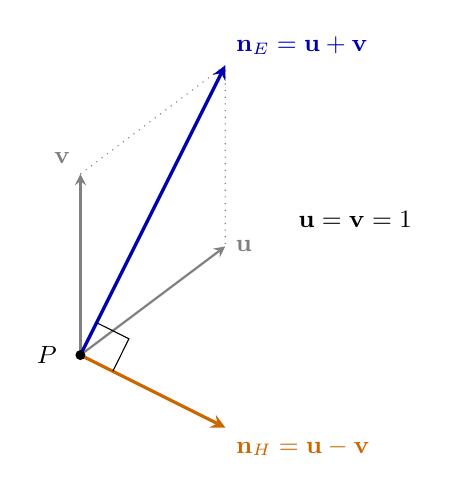
\begin{tikzpicture}[x=2.3cm,y=2.3cm,>=stealth,font=\small]
\coordinate (P) at (0,0);
\draw[gray,dotted] (0,1)--(.8,1.6)--(.8,.6);
\draw[->,gray,thick] (P)--(.8,.6) node[right] {$\mathbf u$};
\draw[->,gray,thick] (P)--(0,1) node[above left] {$\mathbf v$};
\draw[->,blue!70!black,very thick] (P)--(.8,1.6) node[above right] {$\mathbf n_E=\mathbf u+\mathbf v$};
\draw[->,orange!80!black,very thick] (P)--(.8,-.4) node[below right] {$\mathbf n_H=\mathbf u-\mathbf v$};
\draw (.089,.179)--(.268,.09)--(.179,-.089);
\fill (P) circle (1.8pt) node[left=5pt] {$P$};
\node[anchor=west] at (1.15,.75) {$\lVert\mathbf u\rVert=\lVert\mathbf v\rVert=1$};
\end{tikzpicture}
